% Project-authored scaling study with sampled functions and reference points.
% Syntax reference: https://tikz.dev/pgfplots/reference-axis
\documentclass{article}
\usepackage{pgfplots}
\pgfplotsset{compat=1.18}

\title{Algorithm Scaling Study}
\author{Systems Performance Group}
\date{September 2026}

\begin{document}
\maketitle

\section{Comparing growth rates}
The three curves show linear, superlinear, and quadratic growth over problem
sizes from one to sixty-four. The measurements are illustrative operation
counts from a synthetic benchmark. Both axes are logarithmic, making a
power-law relationship visible as an approximately straight line.

\begin{figure}
\centering
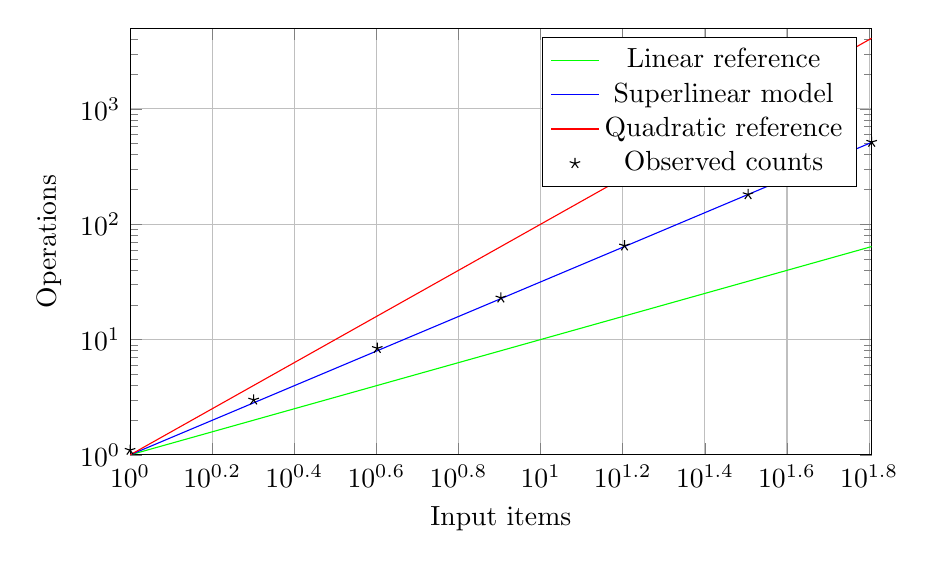
\begin{tikzpicture}
  \begin{loglogaxis}[
    xmin=1,xmax=64,ymin=1,ymax=5000,
    width=11cm,height=7cm,
    xlabel={Input items},ylabel={Operations},
    grid=major,domain=1:64,samples=41]
    \addplot[green] {x};
    \addlegendentry{Linear reference}
    \addplot[blue] {x^1.5};
    \addlegendentry{Superlinear model}
    \addplot[red] {x^2};
    \addlegendentry{Quadratic reference}
    \addplot+[black,only marks] coordinates {
      (1,1.1) (2,3.0) (4,8.4) (8,23.0)
      (16,65.0) (32,181.0) (64,515.0)
    };
    \addlegendentry{Observed counts}
  \end{loglogaxis}
\end{tikzpicture}
\caption{Measured counts against three reference growth laws.}
\label{fig:scaling}
\end{figure}

The observations follow the superlinear curve more closely than either
reference curve. The explicit positive limits also test both log domains.
\end{document}
